\chapter{Metodologia}

Este capítulo apresenta a metodologia empregada no desenvolvimento e na validação da plataforma didática proposta para o estudo de funções de proteção de sistemas elétricos de potência. O procedimento estabelece um fluxo rastreável entre a simulação do evento elétrico, a geração da oscilografia, sua reprodução em bancada e a decisão de proteção. Em síntese, as formas de onda são geradas no MATLAB/Simulink, organizadas no padrão COMTRADE, transferidas para uma ESP32 geradora, convertidas em sinais analógicos por um DAC MCP4728, adquiridas por uma ESP32 receptora e avaliadas por algoritmos embarcados de proteção.

Embora o sistema elétrico simulado seja trifásico, a implementação física analisada neste trabalho é monofásica: um canal de tensão e um canal de corrente, correspondentes à fase selecionada no registro, são reproduzidos e adquiridos. Essa delimitação é compatível com o objetivo de demonstrar, em uma bancada de baixo custo, o encadeamento completo entre falta, oscilografia, grandezas fasoriais e atuação. Os detalhes de implementação, como pinagem, estruturas de dados, protocolo serial e organização interna dos programas, são apresentados no capítulo seguinte.

\section{Caracterização e delimitação da pesquisa}

O trabalho possui natureza aplicada, abordagem experimental e finalidade didática. É aplicado porque propõe uma solução concreta para apoiar o ensino de proteção de sistemas elétricos; experimental porque integra simulação computacional, arquivos de oscilografia, sistemas embarcados, conversão digital-analógica, aquisição analógica e saídas digitais; e didático porque permite observar, em uma mesma plataforma, a relação entre o fenômeno elétrico simulado e a decisão produzida por um relé digital emulado.

A plataforma não pretende substituir relés comerciais nem malas de teste certificadas. Seu propósito é oferecer um ambiente de baixo custo, reconfigurável e repetível para demonstração de conceitos e realização de ensaios acadêmicos. Por essa razão, a metodologia prioriza a rastreabilidade dos parâmetros, a repetibilidade do procedimento e a correspondência entre as grandezas do arquivo COMTRADE e aquelas interpretadas pela unidade receptora.

\section{Arquitetura metodológica da plataforma}

A plataforma é constituída por quatro blocos funcionais: (i) geração das oscilografias; (ii) unidade embarcada de geração; (iii) unidade embarcada de aquisição e proteção; e (iv) indicação da atuação. A Figura \ref{fig:arquitetura-metodologia} apresenta a arquitetura geral e evidencia que o arquivo JSON de configuração conecta logicamente as interfaces de geração e recepção.

\begin{figure}[H]
    \centering
    \caption{Arquitetura funcional da plataforma didática proposta.}
    \label{fig:arquitetura-metodologia}
    \makebox[\textwidth][c]{%
      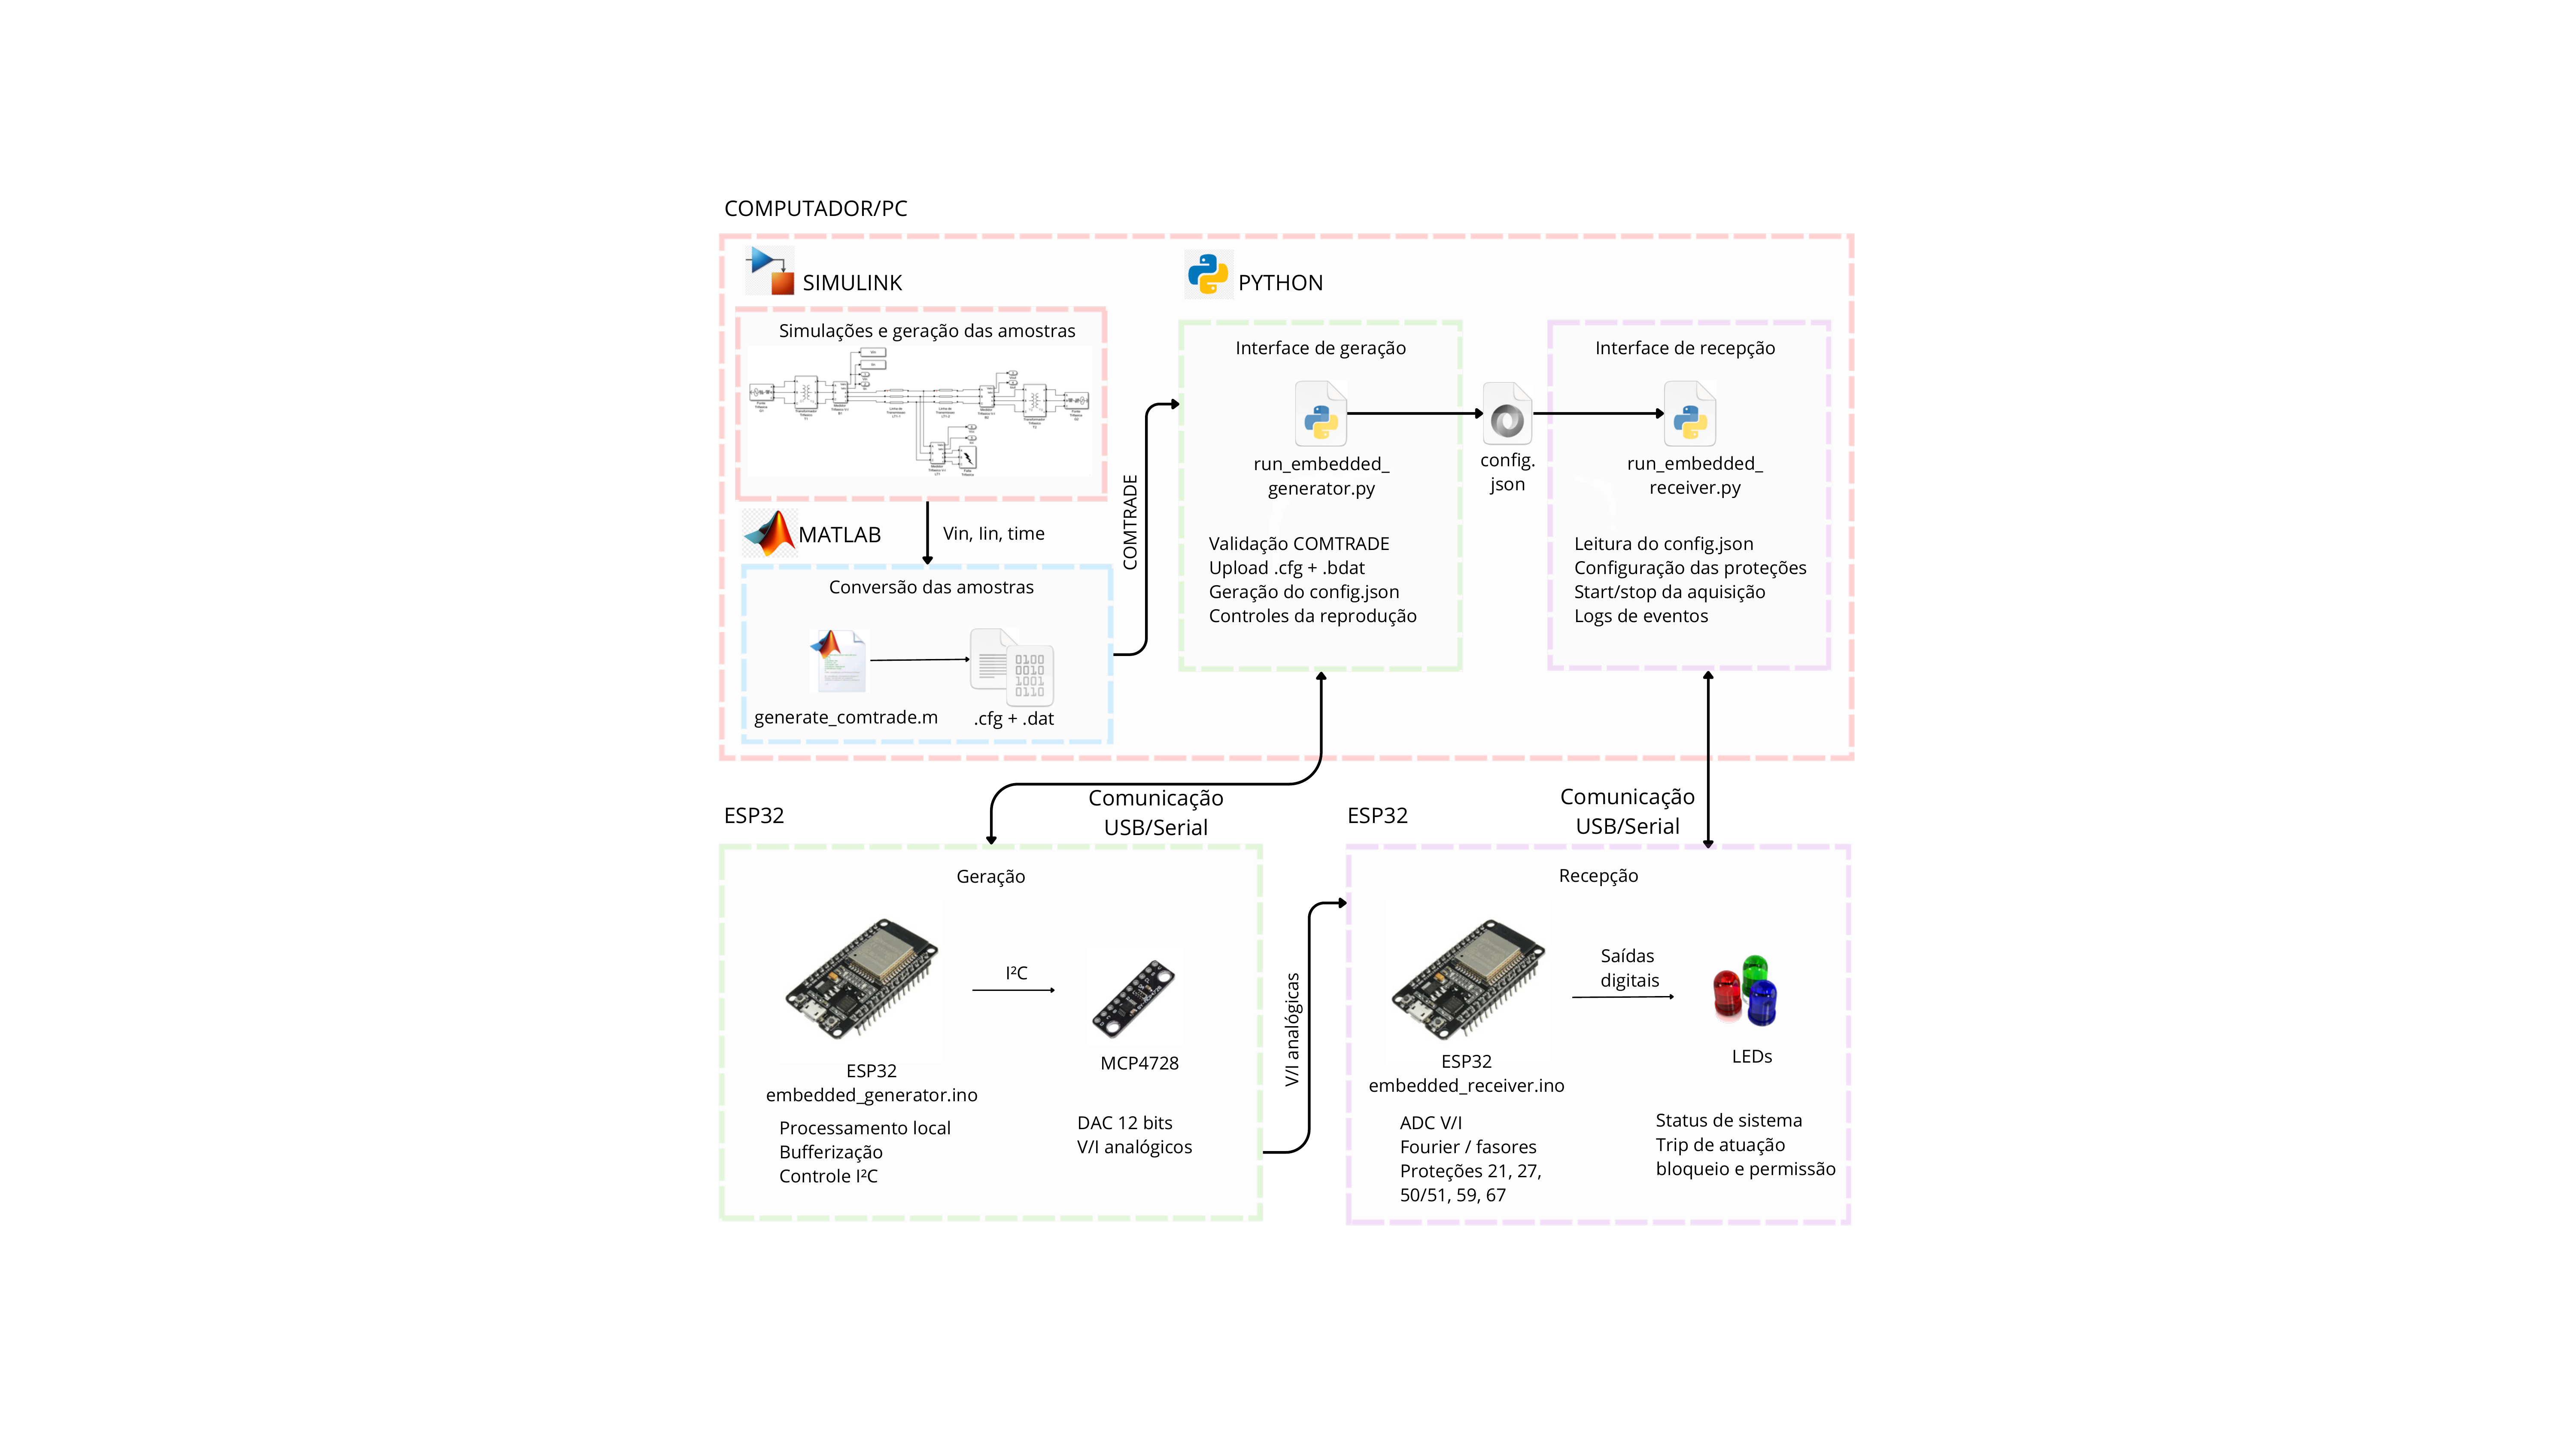
\includegraphics[
          width=\textwidth,
          trim=14cm 4cm 14cm 3cm,
          clip
      ]{figuras/arquitetura_geral_v3_limpo.png}%
    }
    \legend{Fonte: Autoria própria.}
\end{figure}

O fluxo metodológico compreende as seguintes etapas:

\begin{enumerate}
  \item modelagem do sistema elétrico e simulação dos eventos no Simulink;
  \item exportação dos vetores de tempo, tensão e corrente para o MATLAB;
  \item organização das amostras em um registro COMTRADE compatível com a geradora;
  \item validação e transferência do par de arquivos \texttt{.cfg}/\texttt{.bdat};
  \item interpretação do COMTRADE e preparação dos quadros de reprodução na ESP32 geradora;
  \item geração do arquivo \texttt{config.json}, específico para o ensaio processado;
  \item reprodução analógica de tensão e corrente pelo DAC MCP4728;
  \item configuração e aquisição dos sinais pela ESP32 receptora;
  \item estimação da componente fundamental e avaliação das funções de proteção; e
  \item registro dos eventos e indicação dos estados por LEDs e saídas digitais.
\end{enumerate}

Essa sequência separa o domínio de potência simulado do domínio de baixa tensão da bancada. A ligação entre ambos não é feita pela amplitude elétrica física original, mas por fatores de escala documentados e aplicados de forma coerente nas duas unidades embarcadas.

\section{Geração das amostras no MATLAB/Simulink}

A primeira etapa consiste na simulação de um sistema de transmissão em \SI{500}{\kilo\volt}. O modelo contém fontes equivalentes, transformadores trifásicos, dois trechos de linha de transmissão, blocos de medição e um bloco de aplicação de falta. Seu objetivo é produzir, de maneira controlada, sinais de tensão e corrente representativos das condições que se deseja submeter às funções de proteção.

Conforme ilustrado na Figura \ref{fig:modelo-simulink}, a fonte G1 alimenta o sistema por meio do transformador T1. As grandezas são medidas antes e depois dos trechos LT1-1 e LT1-2, e o terminal remoto é representado pelo transformador T2 e pela fonte equivalente G2. O bloco de falta é conectado ao ponto intermediário da linha, o que permite variar a posição e as condições do defeito.

\begin{figure}[H]
  \centering
  \caption{Modelo do sistema elétrico implementado no Simulink.}
  \label{fig:modelo-simulink}
  \makebox[\textwidth][c]{%
    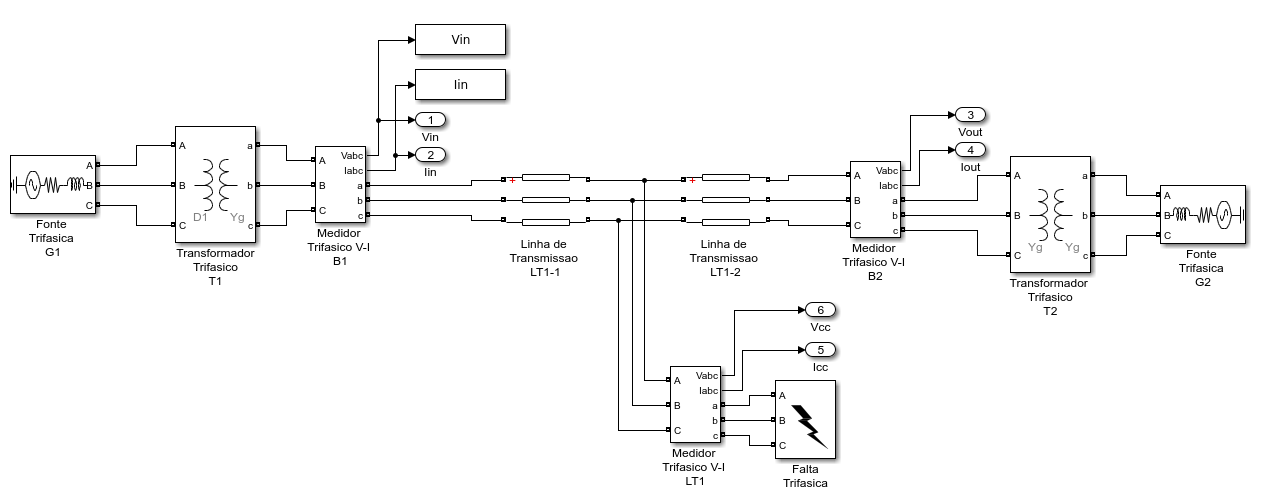
\includegraphics[width=1.10\textwidth]{figuras/modelo_simulink.png}
  }
  \legend{Fonte: Autoria própria.}
\end{figure}

Adotou-se a condição de carregamento de 1 SIL (\textit{Surge Impedance Loading}) como referência operacional comum aos ensaios. A utilização de uma mesma condição de base permite alterar, de forma controlada, apenas os parâmetros relacionados à função de proteção sob avaliação.

Os parâmetros da linha de transmissão são apresentados na Tabela \ref{tab:parametros-linha}. A linha possui comprimento de \SI{190}{\kilo\metre}, com parâmetros de sequência zero e de sequência positiva/negativa.

\begin{table}[H]
  \centering
  \small
  \caption{Parâmetros por unidade de comprimento da linha de transmissão de \SI{500}{\kilo\volt}.}
  \label{tab:parametros-linha}
  \begin{tabular}{lccc}
    \toprule
    Sequência & Resistência & Reatância indutiva & Susceptância \\
    \midrule
    Zero (homopolar) & \SI{0,4352}{\ohm\per\kilo\metre} & \SI{1,4427}{\ohm\per\kilo\metre} & \SI{3,5227}{\micro\siemens\per\kilo\metre} \\
    Positiva/negativa & \SI{0,0161}{\ohm\per\kilo\metre} & \SI{0,2739}{\ohm\per\kilo\metre} & \SI{6,0417}{\micro\siemens\per\kilo\metre} \\
    \bottomrule
  \end{tabular}
  \legend{Fonte: Dados do sistema-teste utilizado nas simulações.}
\end{table}

Os parâmetros das fontes equivalentes, para a condição de 1 SIL, são apresentados nas Tabelas \ref{tab:parametros-gerador} e \ref{tab:parametros-fonte-equivalente}.

\begin{table}[H]
  \centering
  \small
  \caption{Parâmetros do gerador equivalente G1 na condição de 1 SIL.}
  \label{tab:parametros-gerador}
  \begin{tabular}{lcccc}
    \toprule
    Equipamento & Potência & Tensão & Reatância & Resistência \\
    \midrule
    G1 & \SI{1417,5}{\mega\volt\ampere} & $\SI{15,37}{\kilo\volt}\angle \ang{3,41}$ & \SI{0,04317}{\ohm} & \SI{0,001257}{\ohm} \\
    \bottomrule
  \end{tabular}
  \legend{Fonte: Dados do sistema-teste utilizado nas simulações.}
\end{table}

\begin{table}[H]
  \centering
  \small
  \caption{Parâmetros das fontes equivalentes no terminal remoto.}
  \label{tab:parametros-fonte-equivalente}
  \begin{tabular}{lccccc}
    \toprule
    Condição & Tensão & $R_{1\mathrm{th}}$ & $X_{1\mathrm{th}}$ & $R_{0\mathrm{th}}$ & $X_{0\mathrm{th}}$ \\
    \midrule
    Fraca & $\SI{501,27}{\kilo\volt}\angle \ang{-15,97}$ & \SI{7,6980}{\ohm} & \SI{46,188}{\ohm} & \SI{46,188}{\ohm} & \SI{230,9401}{\ohm} \\
    Forte & $\SI{498,70}{\kilo\volt}\angle \ang{-6,51}$ & \SI{1,9245}{\ohm} & \SI{11,5475}{\ohm} & \SI{11,5475}{\ohm} & \SI{57,7349}{\ohm} \\
    \bottomrule
  \end{tabular}
  \legend{Fonte: Dados do sistema-teste utilizado nas simulações.}
\end{table}

Os transformadores T1 e T2 foram representados com conexões $\Delta/Y_g$ e $Y_g/Y_g$, respectivamente. Os parâmetros utilizados são apresentados na Tabela \ref{tab:parametros-transformador}.

\begin{table}[H]
  \centering
  \small
  \caption{Parâmetros dos transformadores empregados no modelo.}
  \label{tab:parametros-transformador}
  \begin{tabular}{lc}
    \toprule
    Parâmetro & Valor \\
    \midrule
    Reatância de dispersão do primário (\SI{15}{\kilo\volt}) & \SI{0,0846}{\ohm} \\
    Reatância de dispersão do secundário (\SI{525}{\kilo\volt}) & \SI{31,3380}{\ohm} \\
    Resistência do primário (\SI{15}{\kilo\volt}) & \SI{0,0030}{\ohm} \\
    Resistência do secundário (\SI{525}{\kilo\volt}) & \SI{0,7950}{\ohm} \\
    \bottomrule
  \end{tabular}
  \legend{Fonte: Dados do sistema-teste utilizado nas simulações.}
\end{table}

Em cada cenário são definidos o tipo, o local e o instante de aplicação da falta, sua duração, a frequência nominal e a taxa de amostragem. Os vetores trifásicos \texttt{Vin}, \texttt{Iin} e o vetor de tempo são enviados ao \textit{workspace} do MATLAB. As Figuras \ref{fig:saida-tensao} e \ref{fig:saida-corrente} apresentam exemplos dessas amostras. A preservação de uma base temporal comum é indispensável para manter a relação de fase entre tensão e corrente, da qual dependem as funções 21 e 67.

\begin{figure}[H]
    \centering
    \caption{Tensões trifásicas obtidas na simulação.}
    \label{fig:saida-tensao}
    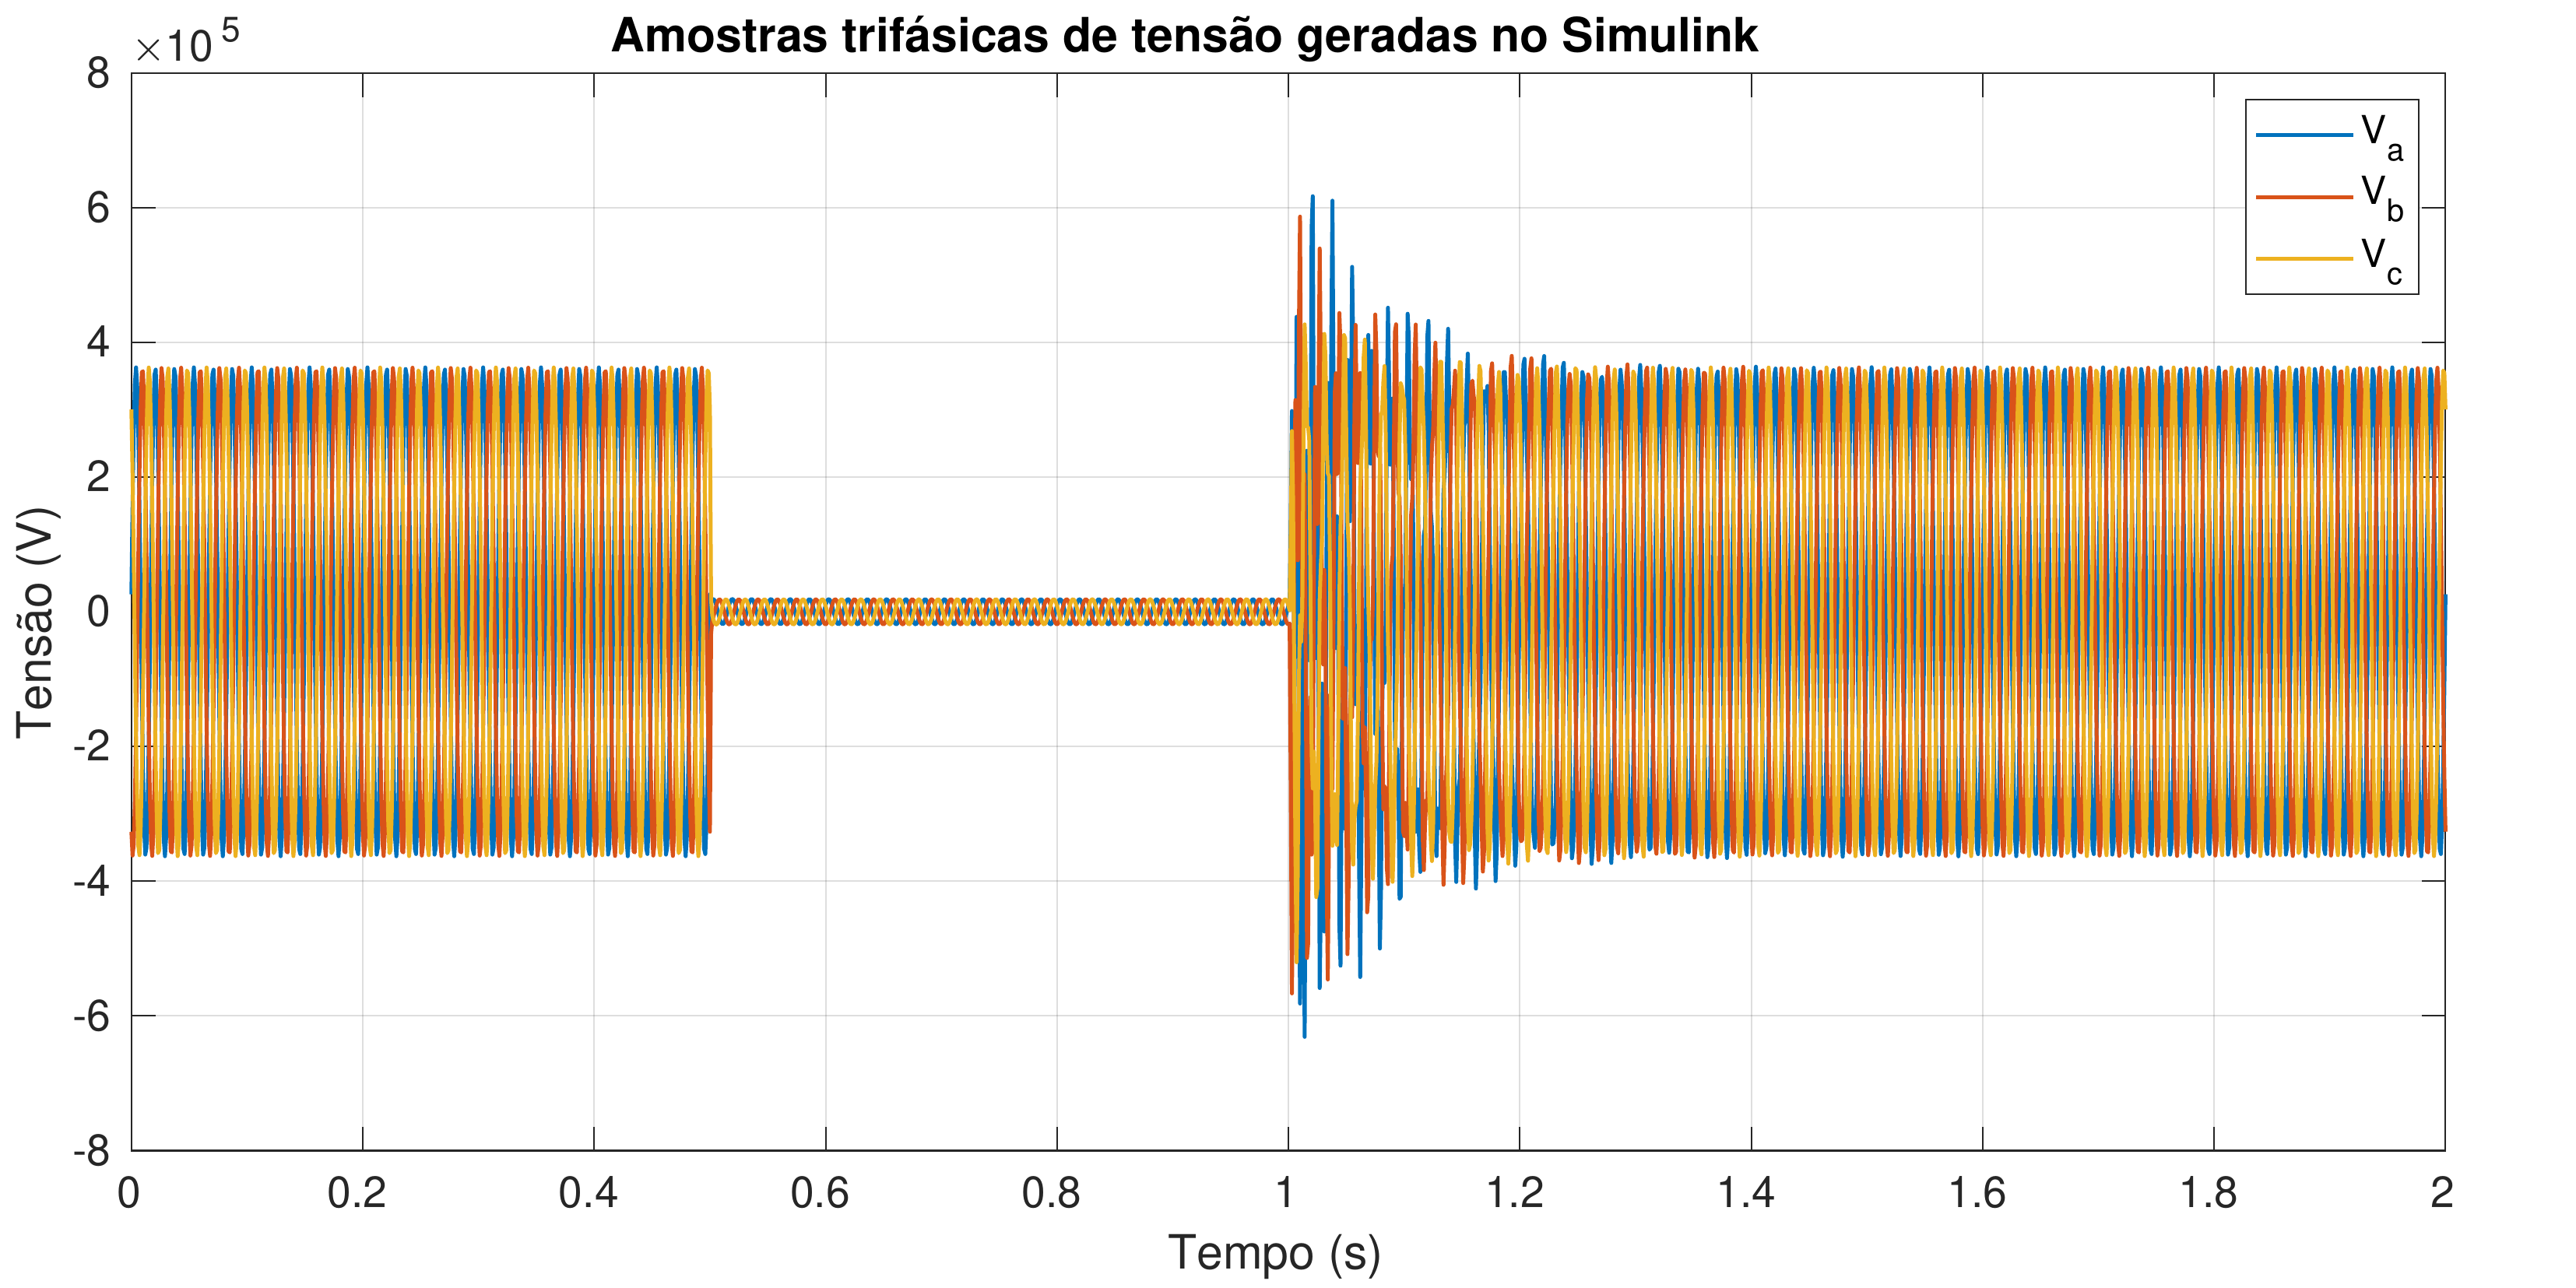
\includegraphics[width=0.95\textwidth]{figuras/simulink_tensao_limpo.png}
    \legend{Fonte: Autoria própria.}
\end{figure}

\begin{figure}[H]
    \centering
    \caption{Correntes trifásicas obtidas na simulação.}
    \label{fig:saida-corrente}
    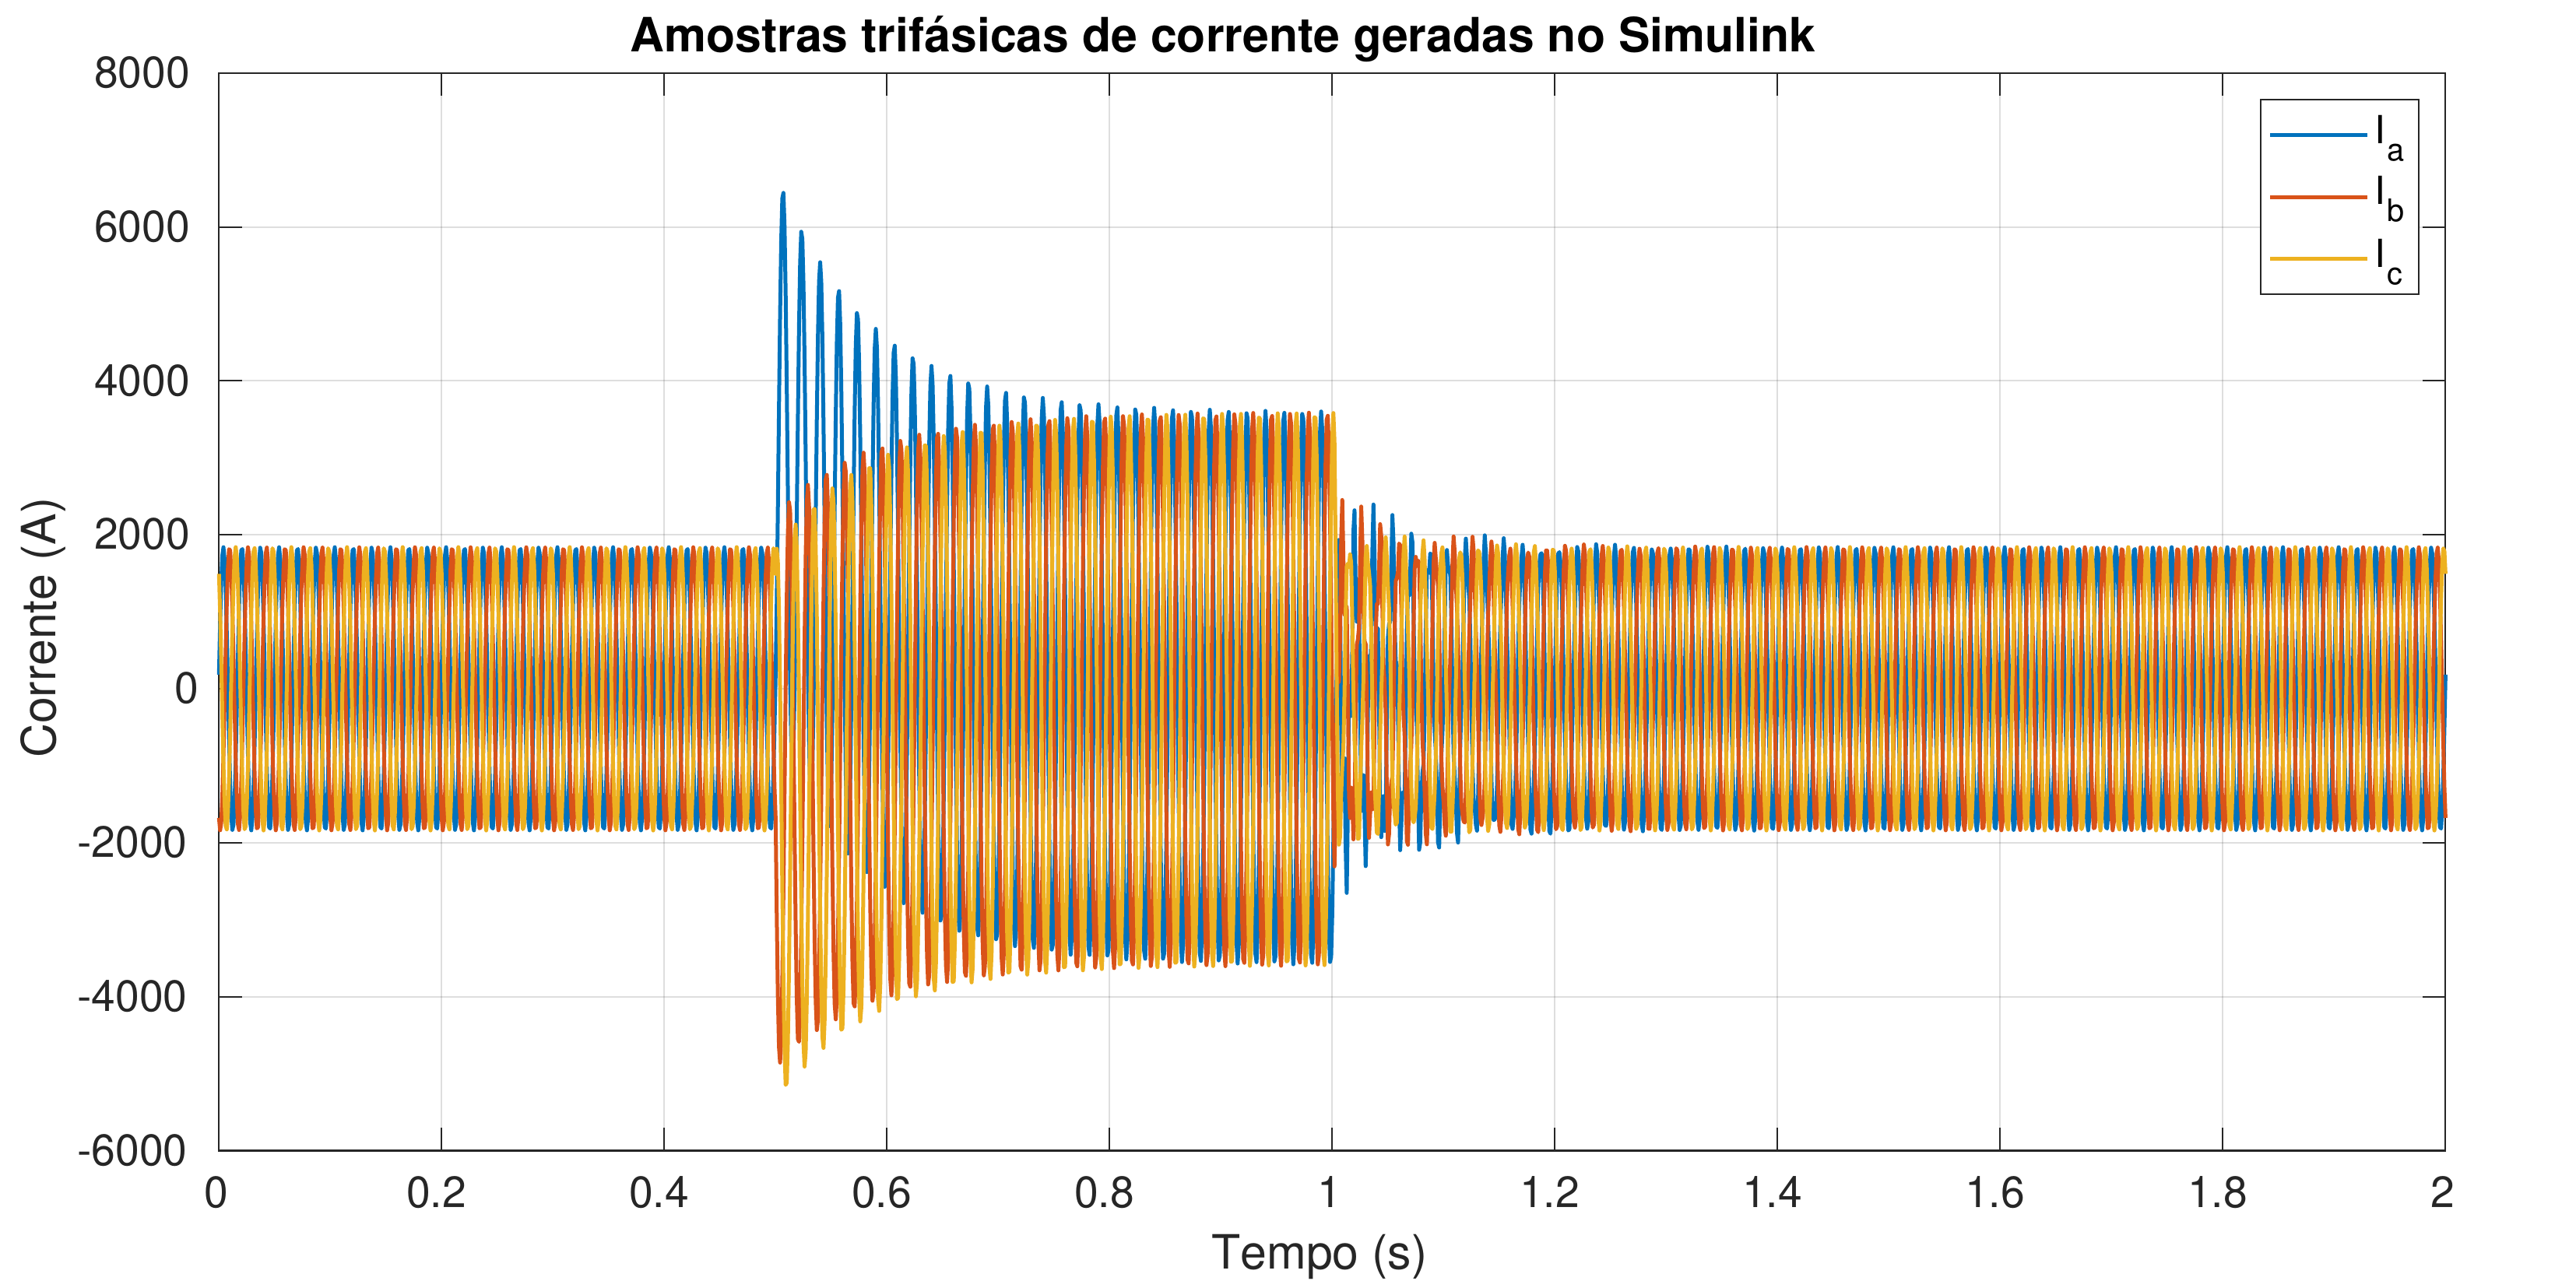
\includegraphics[width=0.95\textwidth]{figuras/simulink_corrente_limpo.png}
    \legend{Fonte: Autoria própria.}
\end{figure}

\subsection{Definição dos cenários de ensaio}

Os cenários foram elaborados de acordo com a função de proteção avaliada. Para as funções 27 e 59, modifica-se a tensão no ponto de medição para que a magnitude fundamental permaneça, durante o tempo requerido, abaixo ou acima do valor de atuação. Para as funções 50 e 51, varia-se a impedância equivalente entre o ponto de medição e a falta, alterando a corrente de curto-circuito. Para a função 21, desloca-se o ponto de falta ao longo da linha, de modo que a impedância aparente $Z=V_1/I_1$ fique dentro ou fora das zonas mho configuradas. Para a supervisão direcional 67, altera-se a defasagem entre G1 e G2 para produzir fluxo de potência direto ou reverso.

\begin{table}[H]
  \centering
  \small
  \caption{Estratégia de geração dos cenários de validação.}
  \label{tab:cenarios-protecao}
  \begin{tabular}{lll}
    \toprule
    Função ANSI & Variável controlada & Condição observada \\
    \midrule
    27 & Tensão no ponto de medição & $V_1$ inferior ao ajuste durante o atraso \\
    59 & Tensão no ponto de medição & $V_1$ superior ao ajuste durante o atraso \\
    50/51 & Impedância até a falta & Corrente acima dos níveis ajustados \\
    21 & Localização da falta & Impedância aparente nas zonas 1 ou 2 \\
    67 & Ângulo entre as fontes & Sentido direto ou reverso da potência \\
    \bottomrule
  \end{tabular}
  \legend{Fonte: Autoria própria.}
\end{table}

\section{Preparação e validação do registro COMTRADE}

O \textit{script} \texttt{generate\_comtrade.m} organiza os vetores do MATLAB e produz um registro COMTRADE com arquivo de configuração \texttt{.cfg} e arquivo de dados. O \texttt{.cfg} descreve o registro, incluindo canais, unidades, fatores de conversão, frequência nominal, taxa de amostragem e formato dos dados; o segundo arquivo contém as amostras e suas marcas de tempo. A adoção do COMTRADE aproxima a plataforma dos procedimentos empregados na análise de oscilografias de sistemas elétricos \cite{ieee_comtrade,iec_60255_24_2013}.

O modelo MATLAB gera originalmente seis canais analógicos trifásicos em formato ASCII. Entretanto, o \textit{firmware} \path{embedded_generator.ino} da unidade geradora processa registros binários e interpreta os dois primeiros canais analógicos como tensão e corrente. Por isso, antes do envio, o registro utilizado na bancada deve ser exportado ou convertido para o par \texttt{.cfg}/\texttt{.bdat} no formato \texttt{BINARY}, contendo como primeiros canais a tensão e a corrente da fase selecionada. Essa adequação de formato e de ordem dos canais é parte explícita do preparo dos dados, e não uma etapa implícita do ensaio.

Antes do \textit{upload}, verificam-se:

\begin{itemize}
  \item a existência e a correspondência entre os arquivos \texttt{.cfg} e \texttt{.bdat};
  \item a declaração do formato \texttt{BINARY} no arquivo \texttt{.cfg};
  \item a presença de, pelo menos, dois canais analógicos, ordenados como tensão e corrente;
  \item as unidades e os coeficientes de conversão dos canais;
  \item a frequência nominal, a taxa de amostragem e o número de registros;
  \item a coerência do tamanho de cada registro binário e das marcas de tempo; e
  \item a compatibilidade da quantidade de amostras com a memória da ESP32.
\end{itemize}

Registros que não atendam a esses critérios não devem prosseguir para o ensaio, pois uma troca de canais ou um fator de conversão incorreto pode produzir atuação aparentemente válida, porém sem significado elétrico.

\section{Transferência e processamento na ESP32 geradora}

O \textit{script} \path{run_embedded_generator.py} estabelece a comunicação USB/serial à taxa de 921600 \textit{baud}, aguarda a sinalização de prontidão, transfere os arquivos em blocos e verifica as confirmações emitidas pela placa. Na arquitetura adotada, o computador atua principalmente como interface de transferência e controle: a interpretação do COMTRADE, o cálculo das referências e a formação dos quadros de reprodução são realizados pelo \textit{firmware} \path{embedded_generator.ino}.

Durante o processamento, a ESP32 determina o leiaute dos registros binários, converte os valores brutos em grandezas de engenharia e estima, a partir dos primeiros ciclos, os picos nominais de tensão e corrente. Em seguida, define limites de representação para preservar a condição de pré-falta e acomodar a elevação das grandezas durante o defeito. A Figura \ref{fig:comandos-geracao} mostra as mensagens de estado emitidas nesse processo.

\begin{figure}[H]
    \centering
    \caption{Transferência e processamento do registro COMTRADE na unidade geradora.}
    \label{fig:comandos-geracao}
    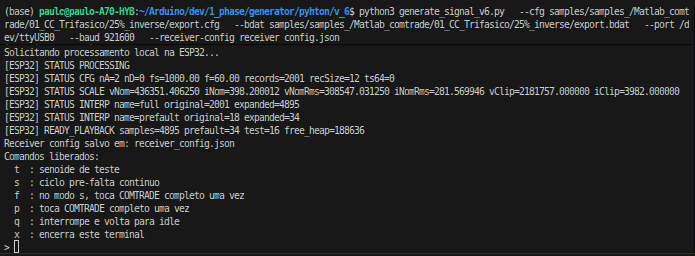
\includegraphics[width=0.95\textwidth]{figuras/terminal_geração.png}
    \legend{Fonte: Autoria própria.}
\end{figure}

\subsection{Arquivo de configuração do receptor}

Após a confirmação de que o registro foi processado, \path{run_embedded_generator.py} cria o arquivo \texttt{config.json}. Esse arquivo não é um acessório opcional: ele constitui o contrato de escala, parametrização e rastreabilidade entre as unidades geradora e receptora. Seu conteúdo vincula a oscilografia selecionada à maneira como ela foi mapeada para o DAC e à forma como deverá ser reconstruída após a aquisição pelo ADC. A sincronização temporal, por sua vez, depende das marcas de tempo reproduzidas pela geradora e da taxa de aquisição configurada na receptora; não há um sinal físico comum de relógio entre as duas placas.

O arquivo contém quatro grupos principais de informações:

\begin{itemize}
  \item \texttt{comtrade}: identificação dos arquivos de origem, quantidade de canais, frequência, taxa de amostragem, número e tamanho dos registros e formato dos dados;
  \item \texttt{dac\_mapping}: tensão de referência, código central, amplitude útil e associação lógica dos canais do DAC;
  \item \texttt{comtrade\_reference}: valores nominais e limites de pico e eficazes calculados para tensão e corrente; e
  \item \texttt{receiver\_recommendation}: mapeamento dos canais de aquisição --- GPIO35 para tensão e GPIO34 para corrente ---, \textit{offsets}, escalas em unidades de engenharia por volt, frequência e taxa de amostragem recomendada.
\end{itemize}

As escalas são calculadas a partir da razão entre o limite de engenharia do registro e a amplitude útil do DAC. Consequentemente, o JSON preserva a equivalência

\begin{equation}
  x_{\mathrm{eng}}=(v_{\mathrm{ADC}}-v_{\mathrm{offset}})k_x,
\end{equation}

em que $x_{\mathrm{eng}}$ representa tensão ou corrente em unidades de engenharia e $k_x$ é o fator de escala correspondente. Se o arquivo for omitido, substituído por outro ensaio ou editado sem controle, as funções de proteção poderão receber magnitudes, valores por unidade e impedâncias aparentes incorretas. Isso comprometeria simultaneamente os ajustes das funções 27, 59, 50, 51 e 21, mesmo que a forma de onda observada permanecesse visualmente senoidal.

Assim, cada par COMTRADE deve permanecer associado ao JSON gerado após seu processamento. Recomenda-se armazená-los na mesma pasta, não reutilizar o JSON de outro cenário e registrar sua identificação junto aos resultados. Antes da execução, também se deve confirmar que o mapeamento declarado no JSON coincide com a pinagem compilada no \textit{firmware} receptor. Na implementação, o \textit{firmware} \path{embedded_receiver.ino} utiliza o GPIO35 para tensão e o GPIO34 para corrente; portanto, qualquer configuração com associação inversa deve ser corrigida antes do ensaio.

Além da associação lógica entre arquivos e canais, a cadeia física DAC--ADC requer uma calibração de ganho da bancada. O \texttt{config.json} descreve a escala ideal usada para converter a oscilografia em tensão analógica e reconstruí-la em unidades de engenharia, mas o ADC interno da ESP32 não apresenta resposta perfeitamente linear nem fundo de escala exatamente igual à referência ideal assumida pelo \textit{firmware}. Por isso, antes dos ensaios que dependem de magnitude absoluta, especialmente 50/51 e 59, a geradora deve permanecer em pré-falta contínua e a receptora deve ser comparada aos valores nominais do JSON pelo comando \texttt{status}. Caso $V_1$ ou $I_1$ de pré-falta não coincidam com os valores nominais, aplicam-se fatores multiplicativos de correção às escalas de tensão e corrente no \textit{script} receptor. Essa correção não altera o COMTRADE nem os valores nominais de referência; ela apenas compensa o ganho efetivo da etapa analógica de aquisição.

\section{Reprodução analógica dos sinais}

O \textit{firmware} \texttt{embedded\_\allowbreak generator.ino} armazena o registro na memória de arquivos da ESP32, constrói os quadros temporizados e comanda o DAC MCP4728 por barramento I\textsuperscript{2}C. O conversor possui resolução de 12 bits e quatro canais \cite{microchip_mcp4728}; nesta aplicação, dois canais representam a tensão e a corrente da fase selecionada.

Como o DAC opera apenas com tensões positivas, as formas de onda alternadas são centralizadas em aproximadamente \SI{1,65}{\volt}. A amplitude útil adotada é de aproximadamente \SI{1,55}{\volt} em torno desse ponto médio, respeitando a faixa de \SIrange{0}{3,3}{\volt}. Os valores que excedem os limites calculados são saturados antes da conversão. A ESP32 também pode interpolar transições entre quadros, reduzindo degraus excessivos na saída.

O \textit{firmware} oferece três condições de reprodução: senoide de teste, ciclo de pré-falta em repetição contínua e execução integral do COMTRADE. A pré-falta contínua permite estabilizar a estimação do \textit{offset}, a detecção de ciclos e, quando habilitada, a normalização do receptor antes da aplicação do evento completo. A Figura \ref{fig:unidade-geradora} apresenta a montagem da unidade geradora.

\begin{figure}[H]
    \centering
    \caption{ESP32 geradora e conversor digital-analógico MCP4728.}
    \label{fig:unidade-geradora}
    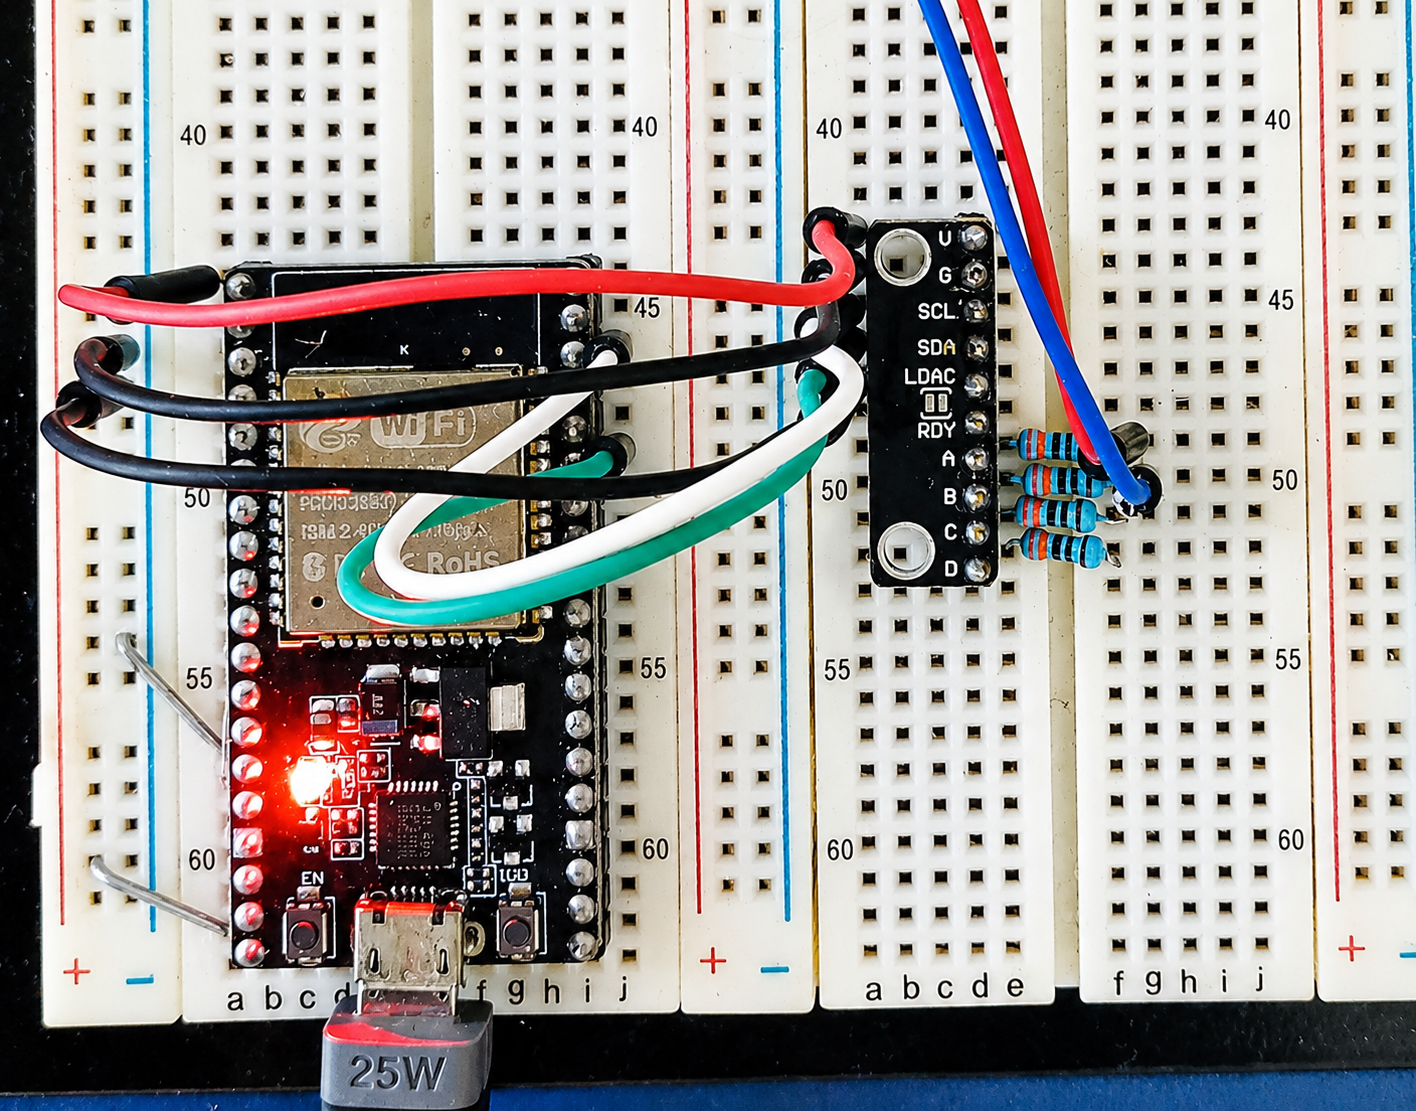
\includegraphics[width=0.75\textwidth]{figuras/esp32_geradora.png}
    \legend{Fonte: Autoria própria.}
\end{figure}

\section{Configuração e aquisição na ESP32 receptora}

O \textit{script} \path{run_embedded_receiver.py} lê o \texttt{config.json}, extrai a taxa de amostragem, as escalas, a frequência de referência e os valores nominais eficazes, combina esses dados com os ajustes de proteção fornecidos na linha de comando e transmite os parâmetros ao \textit{firmware} \path{embedded_receiver.ino}. Cada ajuste recebe uma confirmação individual antes do início da aquisição. A sequência inclui parada preventiva, limpeza dos estados retidos, envio dos parâmetros e comando de início, como mostra a Figura \ref{fig:comandos-protecao}.

\begin{figure}[H]
    \centering
    \caption{Configuração e inicialização da unidade receptora.}
    \label{fig:comandos-protecao}
    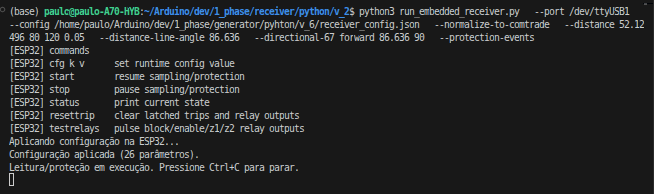
\includegraphics[width=0.95\textwidth]{figuras/terminal_recepção.png}
    \legend{Fonte: Autoria própria.}
\end{figure}

Na implementação atual, a tensão é adquirida pelo GPIO35 e a corrente pelo GPIO34. Para cada instante de amostragem, são realizadas oito leituras do ADC e utilizada sua média. O \textit{firmware} converte os códigos para volts, estima continuamente o nível médio por um filtro de primeira ordem, remove esse \textit{offset} e aplica os fatores de escala provenientes do JSON. Também são sinalizadas condições de saturação, amostras discrepantes, ciclos incompletos e frequência fora da faixa válida.

\begin{figure}[H]
    \centering
    \caption{Unidade embarcada de aquisição, processamento e proteção.}
    \label{fig:unidade-receptora}
    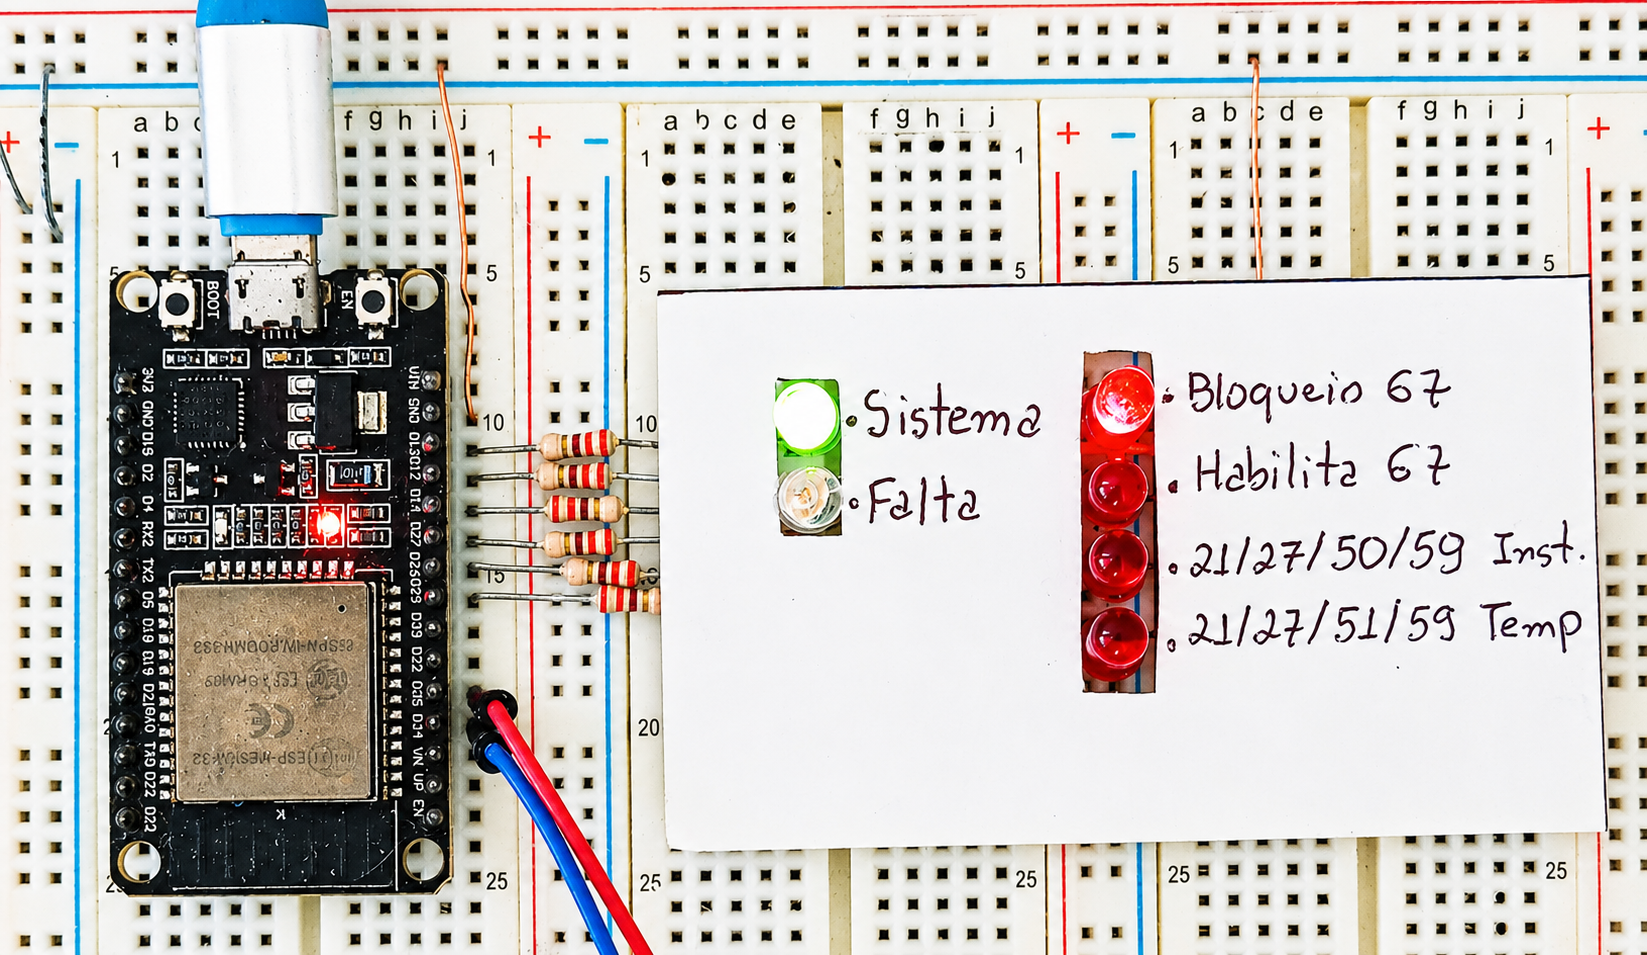
\includegraphics[width=0.85\textwidth]{figuras/esp32_receptora.png}
    \legend{Fonte: Autoria própria.}
\end{figure}

\section{Processamento fasorial e funções de proteção}

Os ciclos elétricos são delimitados pelas passagens ascendentes por zero da tensão, com histerese para reduzir comutações indevidas. Ao término de cada ciclo válido, o \textit{firmware} aplica uma DFT de um ciclo para estimar as magnitudes eficazes e os ângulos da componente fundamental de tensão e corrente. A frequência é obtida do intervalo entre passagens por zero consecutivas. Ciclos com menos de oito amostras ou frequência fora da faixa configurada são invalidados e não alimentam a lógica de proteção.

Opcionalmente, a normalização em relação ao COMTRADE utiliza a mediana de dez ciclos de pré-falta válidos para aproximar as magnitudes medidas dos valores nominais registrados. Esse recurso reduz erros sistemáticos de ganho da cadeia DAC--ADC, mas não substitui o uso correto das escalas nem a verificação de saturação.

As funções implementadas são:

\begin{itemize}
  \item \textbf{ANSI 27}: subtensão em dois estágios, um crítico instantâneo e outro moderado temporizado, com histerese de retorno;
  \item \textbf{ANSI 59}: sobretensão em dois estágios, um crítico instantâneo e outro moderado temporizado, com histerese de retorno;
  \item \textbf{ANSI 50}: sobrecorrente instantânea;
  \item \textbf{ANSI 51}: sobrecorrente de tempo definido, com \textit{pickup} expresso como percentual acima da corrente nominal e atraso ajustável;
  \item \textbf{ANSI 21}: proteção de distância com característica mho, zona 1 instantânea e zona 2 temporizada; e
  \item \textbf{ANSI 67}: supervisão direcional comum às funções 21, 27, 50, 51 e 59.
\end{itemize}

Para a função 21, calcula-se $Z=V_1/I_1$ e decompõe-se a impedância aparente em resistência e reatância. A atuação depende da posição desse ponto no plano $R$--$X$, do alcance percentual das zonas, do ângulo da linha e de uma corrente mínima de supervisão. A zona 1 atua sem atraso intencional, enquanto a zona 2 deve permanecer em \textit{pickup} pelo tempo configurado.

Na versão corrente do \textit{firmware}, a supervisão 67 determina o sentido a partir do sinal da potência ativa de pré-falta, desde que seu módulo ultrapasse o limiar mínimo configurado. O emprego dessa supervisão não constitui uma condição obrigatória para toda aplicação de proteção, pois depende da filosofia adotada. Neste projeto, entretanto, definiu-se que a função 67 pode supervisionar todas as funções atuantes implementadas: 21, 27, 50, 51 e 59. Quando habilitada em conjunto com qualquer uma delas, a função 67 fornece uma permissão comum: o \textit{pickup} continua sendo determinado pelo critério próprio da proteção, mas o \textit{trip} instantâneo ou o início e a continuidade da temporização dependem também da concordância entre o sentido medido e o sentido selecionado (direto ou reverso). Na ausência dessa concordância, a atuação é bloqueada e o temporizador da função supervisionada não avança. A validação metodológica considera esse critério de potência ativa efetivamente executado pelo \textit{firmware}.

\section{Atuação e indicação física}

Quando uma condição de proteção satisfaz os critérios de magnitude, direção e temporização, o \textit{firmware} registra o evento e retém o estado de \textit{trip} até o comando \texttt{resettrip} ou a reinicialização da placa. Os eventos seriais podem indicar \textit{pickup}, temporização, retorno, bloqueio e \textit{trip}, o que permite relacionar a resposta lógica ao instante do evento reproduzido.

As saídas digitais destinadas ao painel indicam: bloqueio imposto pela supervisão 67; permissão direcional fornecida pela função 67; ocorrência de \textit{trip} instantâneo; e ocorrência de \textit{trip} temporizado. A indicação instantânea agrega 21/Z1, os estágios instantâneos de 27 e 59 e a função 50; a temporizada agrega 21/Z2, os estágios temporizados de 27 e 59 e a função 51. Há ainda LEDs para estado do sistema e presença de qualquer \textit{trip}. A origem exata da atuação é identificada pelas mensagens seriais. A Figura \ref{fig:indicacao-leds} apresenta o painel empregado nos ensaios.

\begin{figure}[H]
    \centering
    \caption{Painel de indicação dos estados de proteção.}
    \label{fig:indicacao-leds}
    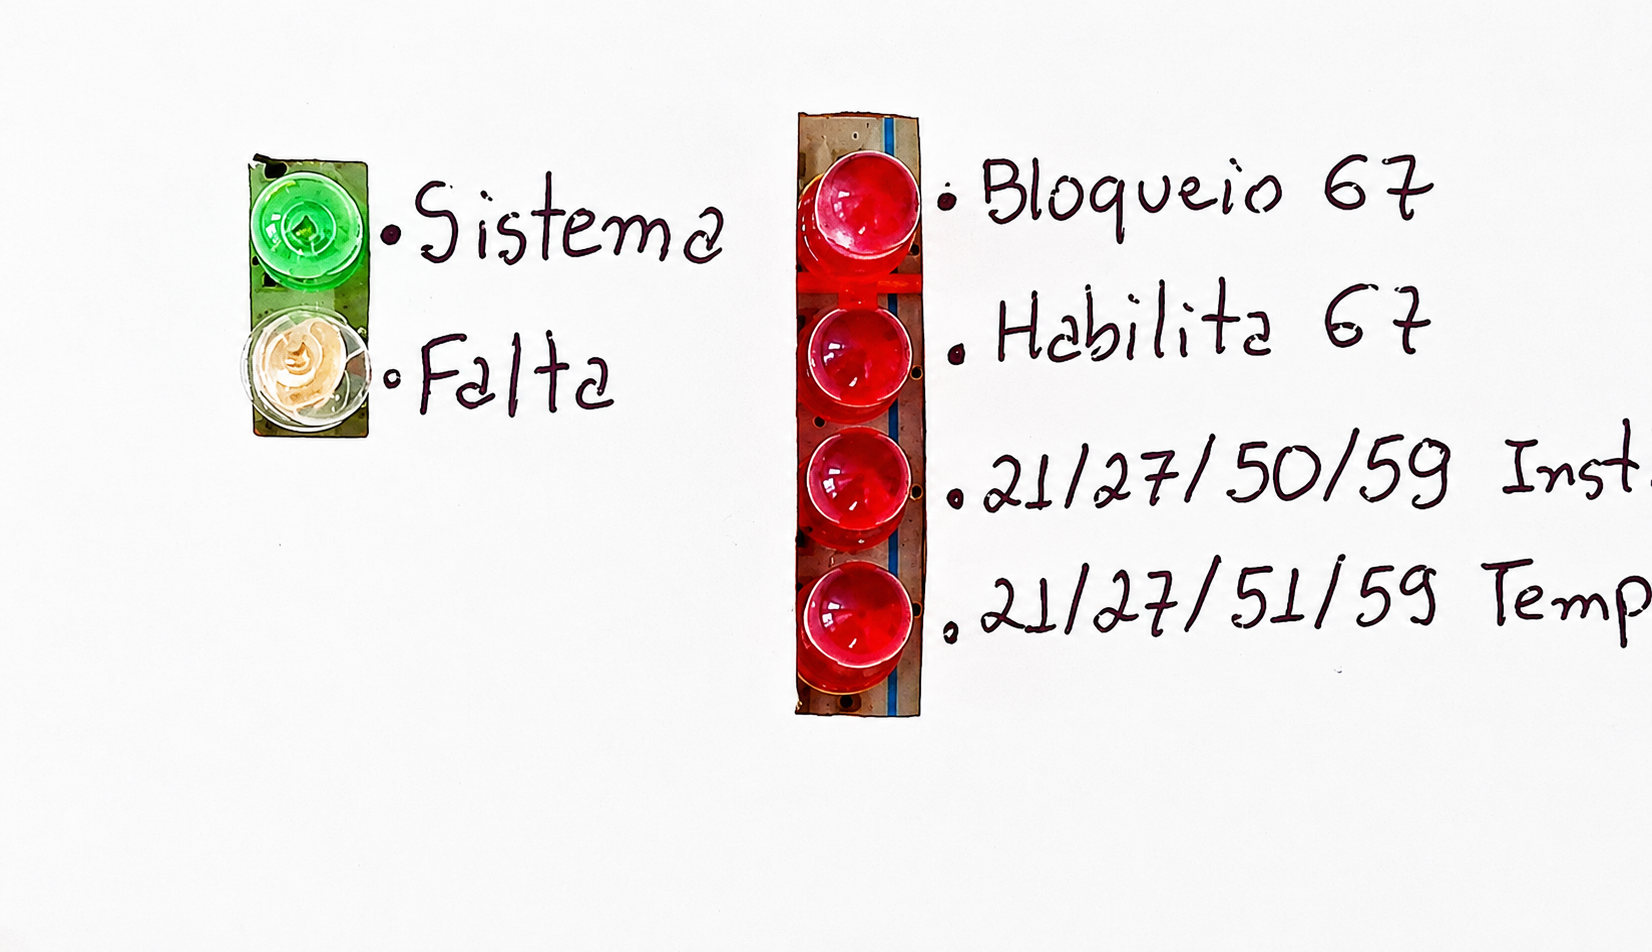
\includegraphics[width=0.75\textwidth]{figuras/painel_leds.png}
    \legend{Fonte: Autoria própria.}
\end{figure}

\section{Procedimento experimental}

Para assegurar a repetibilidade, cada ensaio segue o procedimento abaixo:

\begin{enumerate}
  \item selecionar o cenário simulado e identificar a fase a ser reproduzida;
  \item confirmar que o par \texttt{.cfg}/\texttt{.bdat} é binário, possui tensão e corrente nos dois primeiros canais e corresponde ao cenário escolhido;
  \item transferir os arquivos à ESP32 geradora e aguardar as mensagens de processamento e \texttt{READY\_PLAYBACK};
  \item gerar e arquivar o \texttt{config.json} junto ao COMTRADE, verificando frequência, taxa de amostragem, escalas, valores nominais e associação dos GPIOs;
  \item executar a senoide de teste para verificar continuidade, polaridade, faixa de tensão e ausência de saturação;
  \item iniciar a reprodução em pré-falta contínua na geradora;
  \item iniciar a ESP32 receptora com o JSON do mesmo cenário e com os ajustes da função sob ensaio;
  \item com o evento ainda não liberado, verificar pelo \texttt{status} se $V_1$ e $I_1$ correspondem aos valores nominais do JSON;
  \item quando houver desvio sistemático de ganho, reiniciar a receptora aplicando os fatores \texttt{--v-scale-correction} e \texttt{--i-scale-correction} e repetir a verificação de pré-falta;
  \item manter ciclos de pré-falta até a estabilização do \textit{offset}, da frequência e, quando usada, da normalização;
  \item limpar trips anteriores, iniciar o registro dos eventos e executar uma vez o COMTRADE completo;
  \item observar as mensagens seriais e os LEDs correspondentes a \textit{pickup}, bloqueio, permissão, temporização e \textit{trip}; e
  \item repetir o ensaio para uma condição de atuação e uma condição de não atuação, registrando ajustes, arquivo utilizado e resultado observado.
\end{enumerate}

A Figura \ref{fig:bancada-testes} apresenta a bancada, enquanto a Figura \ref{fig:sistema-completo} detalha a interligação das duas unidades embarcadas, do DAC e do painel de sinalização.

\begin{figure}[H]
    \centering
    \caption{Bancada experimental utilizada na execução dos ensaios.}
    \label{fig:bancada-testes}
    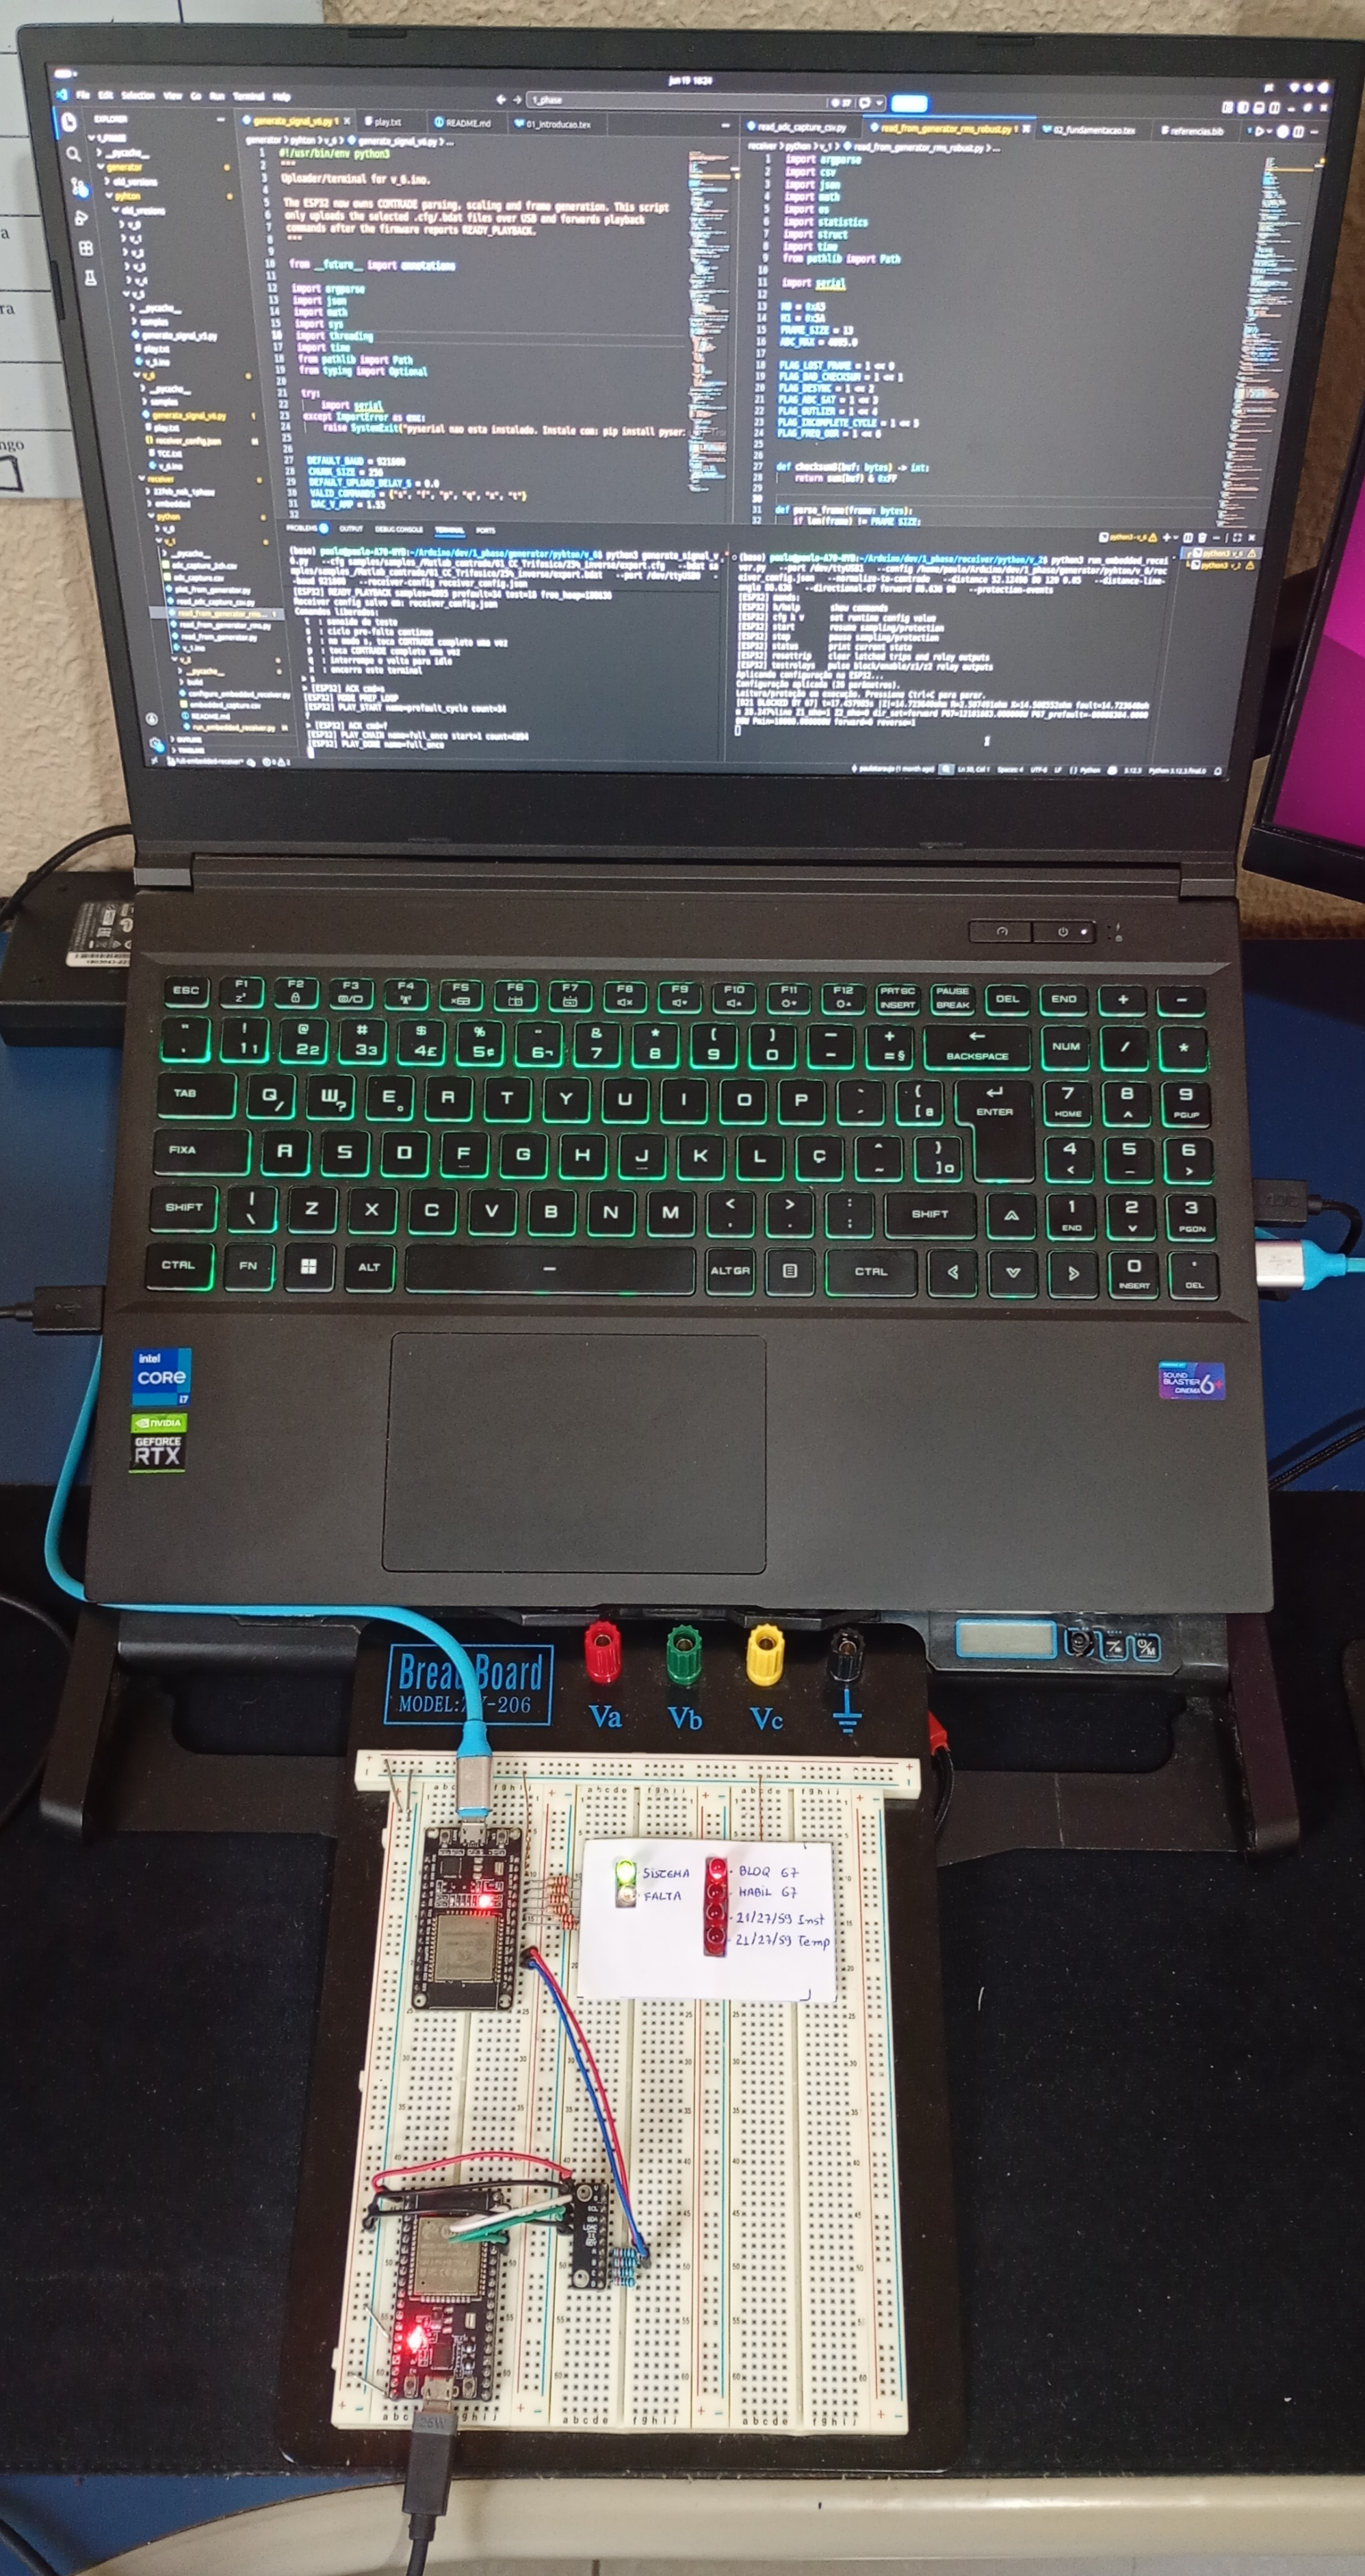
\includegraphics[width=0.72\textwidth]{figuras/bancada_testes.jpg}
    \legend{Fonte: Autoria própria.}
\end{figure}

\begin{figure}[H]
    \centering
    \caption{Montagem completa da plataforma, com geração, conversão, aquisição e sinalização.}
    \label{fig:sistema-completo}
    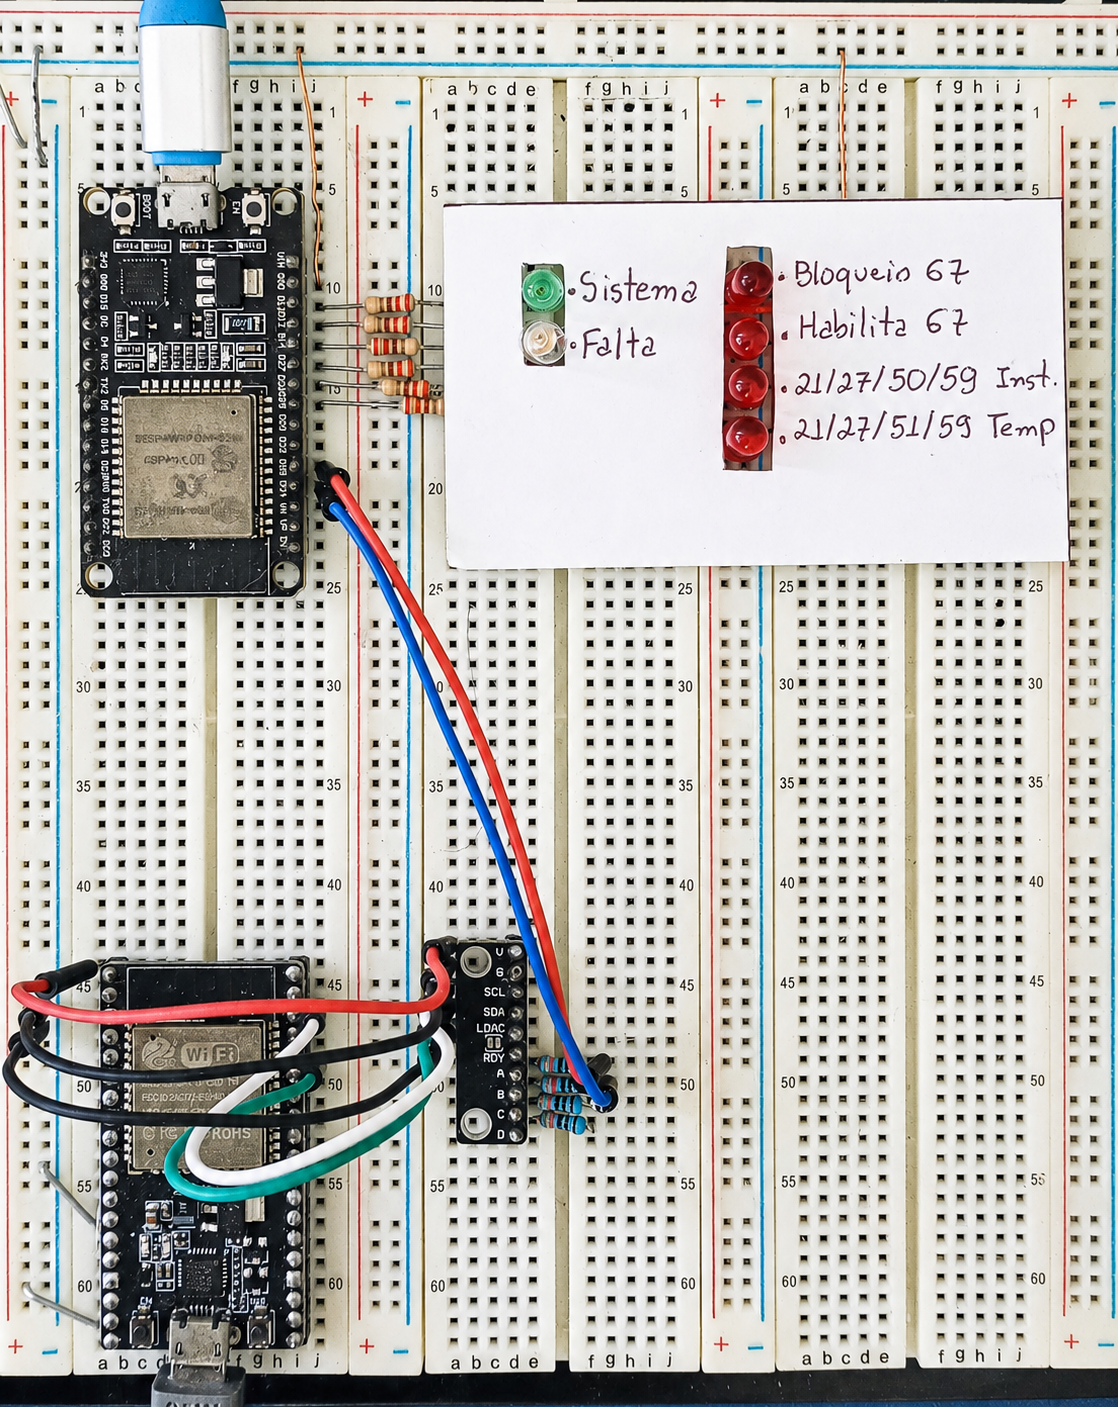
\includegraphics[width=0.72\textwidth]{figuras/bancada_board.png}
    \legend{Fonte: Autoria própria.}
\end{figure}

\section{Critérios de avaliação e controle de qualidade}

A avaliação funcional verifica: aceitação do COMTRADE; conclusão do processamento na geradora; criação do JSON; reprodução sem saturação indevida; aquisição com frequência e número de amostras válidos; coerência das magnitudes fundamentais; e resposta das proteções de acordo com os ajustes. Para cada função, devem ser ensaiadas ao menos uma condição interna e uma externa ao seu limiar, incluindo a verificação do atraso nas funções temporizadas.

A análise dos resultados deve comparar valores esperados e observados, e não apenas registrar que um LED acendeu. Para 27, 59, 50 e 51, comparam-se magnitude, \textit{pickup} e tempo de atuação; para 21, comparam-se a impedância aparente, a zona esperada e o tempo; para 67, comparam-se o sentido selecionado e o estado de permissão ou bloqueio. A condição de não atuação é igualmente necessária para demonstrar seletividade.

Como controles adicionais, recomenda-se registrar, para cada ensaio, o nome dos arquivos COMTRADE e JSON, a versão dos dois \textit{firmwares}, os ajustes enviados, os valores de referência calculados e as mensagens de evento. Também se recomenda validar periodicamente a cadeia analógica com osciloscópio ou instrumento equivalente. Esses registros permitem distinguir falhas do algoritmo de proteção de erros de formato, canal, escala, conexão ou saturação.

Do ponto de vista didático, avalia-se a capacidade da plataforma de tornar observável o encadeamento completo: modelagem da falta, oscilografia, reprodução analógica, aquisição, estimação fasorial, decisão de proteção e indicação física. A contribuição metodológica reside justamente nessa continuidade entre o evento simulado e seu efeito mensurável na bancada.

\section{Conclusão}

Este capítulo descreveu uma metodologia integrada para transformar eventos simulados em ensaios físicos de proteção. O procedimento abrange a geração das amostras no MATLAB/Simulink, a preparação de um COMTRADE binário compatível, seu processamento na ESP32 geradora, a reprodução pelo DAC MCP4728, a aquisição pela ESP32 receptora e a avaliação embarcada das funções ANSI 27, 59, 50, 51, 21 e 67.

O \texttt{config.json} ocupa posição central nesse fluxo, pois preserva a identidade do ensaio e a equivalência de escala entre os domínios digital, analógico e elétrico. Ao associar cada registro COMTRADE aos parâmetros efetivamente utilizados na reprodução e na recepção, o arquivo reduz ambiguidades, favorece a repetibilidade e sustenta a validade dos resultados. Dessa forma, a metodologia estabelece uma base coerente para a implementação detalhada e para a análise experimental apresentadas nos capítulos seguintes.
